% 96-43(96쪽) — $\seg{AD}\parallel\seg{BC}$ 인 사다리꼴 ABCD 와 대각선 AC(원문 「오른쪽 그림」). 스캔 화질이 낮아 TikZ 로 다시 그림.
% 라벨은 원문 것만: 꼭짓점 A·B·C·D, 길이 2·4, $\angle\pt{BAC}=\alpha$, $\angle\pt{ACD}=\beta$. 길이 표시의 점선 호는 원문 꼴.
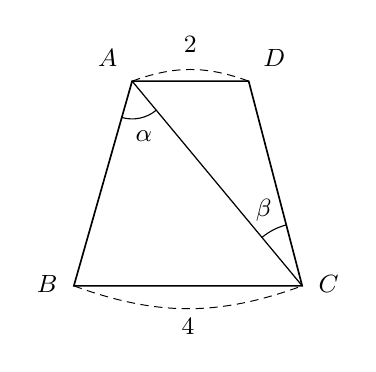
\begin{tikzpicture}[line width=0.6pt, x=1cm, y=1cm]
  \coordinate (B) at (0,0);
  \coordinate (C) at (2.9,0);
  \coordinate (A) at (0.74,2.6);
  \coordinate (D) at (2.22,2.6);
  \draw (A) -- (B) -- (C) -- (D) -- cycle;
  \draw[line width=0.45pt] (A) -- (C);
  % 각 표시
  \draw[line width=0.4pt] ([shift=(-105.9:0.48)]A) arc (-105.9:-50.3:0.48);
  \draw[line width=0.4pt] ([shift=(104.7:0.80)]C) arc (104.7:129.7:0.80);
  \node[font=\small] at (0.890,1.896) {$\alpha$};
  \node[font=\small] at (2.410,0.962) {$\beta$};
  % 길이 표시의 점선 호
  \draw[densely dashed, line width=0.35pt] (A) to[bend left=20] (D);
  \draw[densely dashed, line width=0.35pt] (B) to[bend right=20] (C);
  \node[font=\small] at (1.48,3.06) {$2$};
  \node[font=\small] at (1.45,-0.52) {$4$};
  \node[font=\small, anchor=south east] at (0.68,2.66) {$\pt{A}$};
  \node[font=\small, anchor=south west] at (2.28,2.66) {$\pt{D}$};
  \node[font=\small, anchor=east] at (-0.08,0.02) {$\pt{B}$};
  \node[font=\small, anchor=west] at (2.98,0.02) {$\pt{C}$};
\end{tikzpicture}
